\documentclass[twoside]{book}

% Packages required by doxygen
\usepackage{fixltx2e}
\usepackage{calc}
\usepackage{doxygen}
\usepackage[export]{adjustbox} % also loads graphicx
\usepackage{graphicx}
\usepackage[utf8]{inputenc}
\usepackage{makeidx}
\usepackage{multicol}
\usepackage{multirow}
\PassOptionsToPackage{warn}{textcomp}
\usepackage{textcomp}
\usepackage[nointegrals]{wasysym}
\usepackage[table]{xcolor}

% Font selection
\usepackage[T1]{fontenc}
\usepackage[scaled=.90]{helvet}
\usepackage{courier}
\usepackage{amssymb}
\usepackage{sectsty}
\renewcommand{\familydefault}{\sfdefault}
\allsectionsfont{%
  \fontseries{bc}\selectfont%
  \color{darkgray}%
}
\renewcommand{\DoxyLabelFont}{%
  \fontseries{bc}\selectfont%
  \color{darkgray}%
}
\newcommand{\+}{\discretionary{\mbox{\scriptsize$\hookleftarrow$}}{}{}}

% Page & text layout
\usepackage{geometry}
\geometry{%
  a4paper,%
  top=2.5cm,%
  bottom=2.5cm,%
  left=2.5cm,%
  right=2.5cm%
}
\tolerance=750
\hfuzz=15pt
\hbadness=750
\setlength{\emergencystretch}{15pt}
\setlength{\parindent}{0cm}
\setlength{\parskip}{3ex plus 2ex minus 2ex}
\makeatletter
\renewcommand{\paragraph}{%
  \@startsection{paragraph}{4}{0ex}{-1.0ex}{1.0ex}{%
    \normalfont\normalsize\bfseries\SS@parafont%
  }%
}
\renewcommand{\subparagraph}{%
  \@startsection{subparagraph}{5}{0ex}{-1.0ex}{1.0ex}{%
    \normalfont\normalsize\bfseries\SS@subparafont%
  }%
}
\makeatother

% Headers & footers
\usepackage{fancyhdr}
\pagestyle{fancyplain}
\fancyhead[LE]{\fancyplain{}{\bfseries\thepage}}
\fancyhead[CE]{\fancyplain{}{}}
\fancyhead[RE]{\fancyplain{}{\bfseries\leftmark}}
\fancyhead[LO]{\fancyplain{}{\bfseries\rightmark}}
\fancyhead[CO]{\fancyplain{}{}}
\fancyhead[RO]{\fancyplain{}{\bfseries\thepage}}
\fancyfoot[LE]{\fancyplain{}{}}
\fancyfoot[CE]{\fancyplain{}{}}
\fancyfoot[RE]{\fancyplain{}{\bfseries\scriptsize Generated by Doxygen }}
\fancyfoot[LO]{\fancyplain{}{\bfseries\scriptsize Generated by Doxygen }}
\fancyfoot[CO]{\fancyplain{}{}}
\fancyfoot[RO]{\fancyplain{}{}}
\renewcommand{\footrulewidth}{0.4pt}
\renewcommand{\chaptermark}[1]{%
  \markboth{#1}{}%
}
\renewcommand{\sectionmark}[1]{%
  \markright{\thesection\ #1}%
}

% Indices & bibliography
\usepackage{natbib}
\usepackage[titles]{tocloft}
\setcounter{tocdepth}{3}
\setcounter{secnumdepth}{5}
\makeindex

% Hyperlinks (required, but should be loaded last)
\usepackage{ifpdf}
\ifpdf
  \usepackage[pdftex,pagebackref=true]{hyperref}
\else
  \usepackage[ps2pdf,pagebackref=true]{hyperref}
\fi
\hypersetup{%
  colorlinks=true,%
  linkcolor=blue,%
  citecolor=blue,%
  unicode%
}

% Custom commands
\newcommand{\clearemptydoublepage}{%
  \newpage{\pagestyle{empty}\cleardoublepage}%
}

\usepackage{caption}
\captionsetup{labelsep=space,justification=centering,font={bf},singlelinecheck=off,skip=4pt,position=top}

%===== C O N T E N T S =====

\begin{document}

% Titlepage & ToC
\hypersetup{pageanchor=false,
             bookmarksnumbered=true,
             pdfencoding=unicode
            }
\pagenumbering{alph}
\begin{titlepage}
\vspace*{7cm}
\begin{center}%
{\Large My Project }\\
\vspace*{1cm}
{\large Generated by Doxygen 1.8.13}\\
\end{center}
\end{titlepage}
\clearemptydoublepage
\pagenumbering{roman}
\tableofcontents
\clearemptydoublepage
\pagenumbering{arabic}
\hypersetup{pageanchor=true}

%--- Begin generated contents ---
\chapter{Hierarchical Index}
\section{Class Hierarchy}
This inheritance list is sorted roughly, but not completely, alphabetically\+:\begin{DoxyCompactList}
\item Test\+Case\begin{DoxyCompactList}
\item \contentsline{section}{pruebas.\+Test\+UM}{\pageref{classpruebas_1_1_test_u_m}}{}
\end{DoxyCompactList}
\end{DoxyCompactList}

\chapter{Class Index}
\section{Class List}
Here are the classes, structs, unions and interfaces with brief descriptions\+:\begin{DoxyCompactList}
\item\contentsline{section}{\hyperlink{classpruebas_1_1_test_u_m}{pruebas.\+Test\+UM} }{\pageref{classpruebas_1_1_test_u_m}}{}
\end{DoxyCompactList}

\chapter{Class Documentation}
\hypertarget{classpruebas_1_1_test_u_m}{}\section{pruebas.\+Test\+UM Class Reference}
\label{classpruebas_1_1_test_u_m}\index{pruebas.\+Test\+UM@{pruebas.\+Test\+UM}}
Inheritance diagram for pruebas.\+Test\+UM\+:\begin{figure}[H]
\begin{center}
\leavevmode
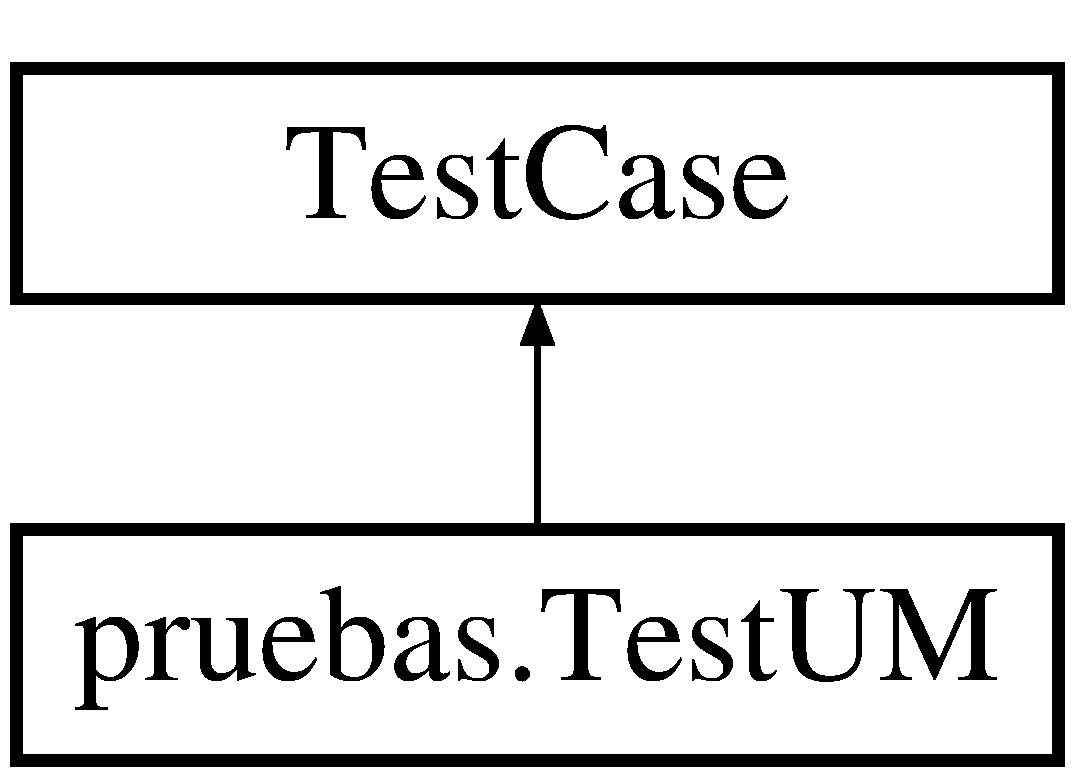
\includegraphics[height=2.000000cm]{classpruebas_1_1_test_u_m}
\end{center}
\end{figure}
\subsection*{Public Member Functions}
\begin{DoxyCompactItemize}
\item 
\mbox{\Hypertarget{classpruebas_1_1_test_u_m_abf7b7300fd629dbef481ff2911f52c44}\label{classpruebas_1_1_test_u_m_abf7b7300fd629dbef481ff2911f52c44}} 
def {\bfseries set\+Up\+Class} (cls)
\item 
\mbox{\Hypertarget{classpruebas_1_1_test_u_m_a9975a254d78eacbd716dd6caba80e243}\label{classpruebas_1_1_test_u_m_a9975a254d78eacbd716dd6caba80e243}} 
def {\bfseries tear\+Down\+Class} (cls)
\item 
\mbox{\Hypertarget{classpruebas_1_1_test_u_m_a977b0959979bf20a4e5e5ecc8e282e30}\label{classpruebas_1_1_test_u_m_a977b0959979bf20a4e5e5ecc8e282e30}} 
def {\bfseries set\+Up} (self)
\item 
\mbox{\Hypertarget{classpruebas_1_1_test_u_m_a0c5a9ed1a1b48a938c7b0f888cbd49f1}\label{classpruebas_1_1_test_u_m_a0c5a9ed1a1b48a938c7b0f888cbd49f1}} 
def {\bfseries tear\+Down} (self)
\item 
def \hyperlink{classpruebas_1_1_test_u_m_a4cecf42b50d10428f2e5c1efca0ce59c}{test\+\_\+index\+\_\+status\+\_\+code} (self)
\item 
def \hyperlink{classpruebas_1_1_test_u_m_a152091a0b91cda976f0ef41a6feef968}{test\+\_\+crear\+\_\+status\+\_\+code} (self)
\item 
def \hyperlink{classpruebas_1_1_test_u_m_a3aa8f257e52cba3f778181f02241ce63}{test\+\_\+generar\+\_\+status\+\_\+code} (self)
\item 
def \hyperlink{classpruebas_1_1_test_u_m_a775d549dfd6d3b2822c5e1579552f6a8}{test\+\_\+predecir\+\_\+status\+\_\+code} (self)
\item 
def \hyperlink{classpruebas_1_1_test_u_m_af0e1b161b7a46c48fe74e9cda7d5cd4c}{test\+\_\+cargar\+\_\+status\+\_\+code} (self)
\item 
def \hyperlink{classpruebas_1_1_test_u_m_a0cda9b35bc5adad4dc7d08c1c6b4bfa8}{test\+\_\+predecir\+\_\+modelo\+\_\+response} (self)
\item 
def \hyperlink{classpruebas_1_1_test_u_m_aeb181c390d170aed40acc8de970abfe1}{test\+\_\+crear\+\_\+csv} (self)
\end{DoxyCompactItemize}
\subsection*{Public Attributes}
\begin{DoxyCompactItemize}
\item 
\mbox{\Hypertarget{classpruebas_1_1_test_u_m_a3dcc06583ad34b984a1daa5ada38bb15}\label{classpruebas_1_1_test_u_m_a3dcc06583ad34b984a1daa5ada38bb15}} 
{\bfseries app}
\end{DoxyCompactItemize}
\subsection*{Static Public Attributes}
\begin{DoxyCompactItemize}
\item 
\mbox{\Hypertarget{classpruebas_1_1_test_u_m_adde7f78dcf948e48a407b7231f8a970f}\label{classpruebas_1_1_test_u_m_adde7f78dcf948e48a407b7231f8a970f}} 
{\bfseries vgg\+\_\+model} = None
\end{DoxyCompactItemize}


\subsection{Member Function Documentation}
\mbox{\Hypertarget{classpruebas_1_1_test_u_m_af0e1b161b7a46c48fe74e9cda7d5cd4c}\label{classpruebas_1_1_test_u_m_af0e1b161b7a46c48fe74e9cda7d5cd4c}} 
\index{pruebas\+::\+Test\+UM@{pruebas\+::\+Test\+UM}!test\+\_\+cargar\+\_\+status\+\_\+code@{test\+\_\+cargar\+\_\+status\+\_\+code}}
\index{test\+\_\+cargar\+\_\+status\+\_\+code@{test\+\_\+cargar\+\_\+status\+\_\+code}!pruebas\+::\+Test\+UM@{pruebas\+::\+Test\+UM}}
\subsubsection{\texorpdfstring{test\+\_\+cargar\+\_\+status\+\_\+code()}{test\_cargar\_status\_code()}}
{\footnotesize\ttfamily def pruebas.\+Test\+U\+M.\+test\+\_\+cargar\+\_\+status\+\_\+code (\begin{DoxyParamCaption}\item[{}]{self }\end{DoxyParamCaption})}

\begin{DoxyVerb}Funcion para probar la respuesta al url: /cargar
\end{DoxyVerb}
 \mbox{\Hypertarget{classpruebas_1_1_test_u_m_aeb181c390d170aed40acc8de970abfe1}\label{classpruebas_1_1_test_u_m_aeb181c390d170aed40acc8de970abfe1}} 
\index{pruebas\+::\+Test\+UM@{pruebas\+::\+Test\+UM}!test\+\_\+crear\+\_\+csv@{test\+\_\+crear\+\_\+csv}}
\index{test\+\_\+crear\+\_\+csv@{test\+\_\+crear\+\_\+csv}!pruebas\+::\+Test\+UM@{pruebas\+::\+Test\+UM}}
\subsubsection{\texorpdfstring{test\+\_\+crear\+\_\+csv()}{test\_crear\_csv()}}
{\footnotesize\ttfamily def pruebas.\+Test\+U\+M.\+test\+\_\+crear\+\_\+csv (\begin{DoxyParamCaption}\item[{}]{self }\end{DoxyParamCaption})}

\begin{DoxyVerb}Funcion para probar la funcion de generacion de archivos .csv
Simula una peticion GET
\end{DoxyVerb}
 \mbox{\Hypertarget{classpruebas_1_1_test_u_m_a152091a0b91cda976f0ef41a6feef968}\label{classpruebas_1_1_test_u_m_a152091a0b91cda976f0ef41a6feef968}} 
\index{pruebas\+::\+Test\+UM@{pruebas\+::\+Test\+UM}!test\+\_\+crear\+\_\+status\+\_\+code@{test\+\_\+crear\+\_\+status\+\_\+code}}
\index{test\+\_\+crear\+\_\+status\+\_\+code@{test\+\_\+crear\+\_\+status\+\_\+code}!pruebas\+::\+Test\+UM@{pruebas\+::\+Test\+UM}}
\subsubsection{\texorpdfstring{test\+\_\+crear\+\_\+status\+\_\+code()}{test\_crear\_status\_code()}}
{\footnotesize\ttfamily def pruebas.\+Test\+U\+M.\+test\+\_\+crear\+\_\+status\+\_\+code (\begin{DoxyParamCaption}\item[{}]{self }\end{DoxyParamCaption})}

\begin{DoxyVerb}Funcion para probar la respuesta al url: /crear
\end{DoxyVerb}
 \mbox{\Hypertarget{classpruebas_1_1_test_u_m_a3aa8f257e52cba3f778181f02241ce63}\label{classpruebas_1_1_test_u_m_a3aa8f257e52cba3f778181f02241ce63}} 
\index{pruebas\+::\+Test\+UM@{pruebas\+::\+Test\+UM}!test\+\_\+generar\+\_\+status\+\_\+code@{test\+\_\+generar\+\_\+status\+\_\+code}}
\index{test\+\_\+generar\+\_\+status\+\_\+code@{test\+\_\+generar\+\_\+status\+\_\+code}!pruebas\+::\+Test\+UM@{pruebas\+::\+Test\+UM}}
\subsubsection{\texorpdfstring{test\+\_\+generar\+\_\+status\+\_\+code()}{test\_generar\_status\_code()}}
{\footnotesize\ttfamily def pruebas.\+Test\+U\+M.\+test\+\_\+generar\+\_\+status\+\_\+code (\begin{DoxyParamCaption}\item[{}]{self }\end{DoxyParamCaption})}

\begin{DoxyVerb}Funcion para probar la respuesta al url: /generar
\end{DoxyVerb}
 \mbox{\Hypertarget{classpruebas_1_1_test_u_m_a4cecf42b50d10428f2e5c1efca0ce59c}\label{classpruebas_1_1_test_u_m_a4cecf42b50d10428f2e5c1efca0ce59c}} 
\index{pruebas\+::\+Test\+UM@{pruebas\+::\+Test\+UM}!test\+\_\+index\+\_\+status\+\_\+code@{test\+\_\+index\+\_\+status\+\_\+code}}
\index{test\+\_\+index\+\_\+status\+\_\+code@{test\+\_\+index\+\_\+status\+\_\+code}!pruebas\+::\+Test\+UM@{pruebas\+::\+Test\+UM}}
\subsubsection{\texorpdfstring{test\+\_\+index\+\_\+status\+\_\+code()}{test\_index\_status\_code()}}
{\footnotesize\ttfamily def pruebas.\+Test\+U\+M.\+test\+\_\+index\+\_\+status\+\_\+code (\begin{DoxyParamCaption}\item[{}]{self }\end{DoxyParamCaption})}

\begin{DoxyVerb}Funcion para probar la respuesta al url: /index
\end{DoxyVerb}
 \mbox{\Hypertarget{classpruebas_1_1_test_u_m_a0cda9b35bc5adad4dc7d08c1c6b4bfa8}\label{classpruebas_1_1_test_u_m_a0cda9b35bc5adad4dc7d08c1c6b4bfa8}} 
\index{pruebas\+::\+Test\+UM@{pruebas\+::\+Test\+UM}!test\+\_\+predecir\+\_\+modelo\+\_\+response@{test\+\_\+predecir\+\_\+modelo\+\_\+response}}
\index{test\+\_\+predecir\+\_\+modelo\+\_\+response@{test\+\_\+predecir\+\_\+modelo\+\_\+response}!pruebas\+::\+Test\+UM@{pruebas\+::\+Test\+UM}}
\subsubsection{\texorpdfstring{test\+\_\+predecir\+\_\+modelo\+\_\+response()}{test\_predecir\_modelo\_response()}}
{\footnotesize\ttfamily def pruebas.\+Test\+U\+M.\+test\+\_\+predecir\+\_\+modelo\+\_\+response (\begin{DoxyParamCaption}\item[{}]{self }\end{DoxyParamCaption})}

\begin{DoxyVerb}Funcion para probar las funciones de prediccion
Simula una peticion POST en la que le envia la imagen perro.jpg
\end{DoxyVerb}
 \mbox{\Hypertarget{classpruebas_1_1_test_u_m_a775d549dfd6d3b2822c5e1579552f6a8}\label{classpruebas_1_1_test_u_m_a775d549dfd6d3b2822c5e1579552f6a8}} 
\index{pruebas\+::\+Test\+UM@{pruebas\+::\+Test\+UM}!test\+\_\+predecir\+\_\+status\+\_\+code@{test\+\_\+predecir\+\_\+status\+\_\+code}}
\index{test\+\_\+predecir\+\_\+status\+\_\+code@{test\+\_\+predecir\+\_\+status\+\_\+code}!pruebas\+::\+Test\+UM@{pruebas\+::\+Test\+UM}}
\subsubsection{\texorpdfstring{test\+\_\+predecir\+\_\+status\+\_\+code()}{test\_predecir\_status\_code()}}
{\footnotesize\ttfamily def pruebas.\+Test\+U\+M.\+test\+\_\+predecir\+\_\+status\+\_\+code (\begin{DoxyParamCaption}\item[{}]{self }\end{DoxyParamCaption})}

\begin{DoxyVerb}Funcion para probar la respuesta al url: /predecir
\end{DoxyVerb}
 

The documentation for this class was generated from the following file\+:\begin{DoxyCompactItemize}
\item 
pruebas.\+py\end{DoxyCompactItemize}

%--- End generated contents ---

% Index
\backmatter
\newpage
\phantomsection
\clearemptydoublepage
\addcontentsline{toc}{chapter}{Index}
\printindex

\end{document}
